\section{Results and Discussion}
The raw data would show the intensity of light, measured as the absolute amount of photons, as a function of the wavelength. This makes the spectrum dependent on the initial wavelength of the laser light. A Raman spectrum is not dependent on the initial wavelength and shows the intensity as a function of the difference in wavenumber of the observed photons to the initial laser light, the Raman shift. In order to be able to compare the experimental results to literature, certain calculations have to be performed.

\subsection{Evaluation of the Measured Data}

    As mentioned in Section \ref{mat_met}, the data is exported as a text file with pairs of numbers. The first number refers to the wavelength at which an intensity was recorded, the second number specifies that intensity. The specific wavelengths reported stay the same for all measurements, since they are predefined by the spectrometer.


    \begin{equation}
        \widetilde{\nu} = \frac{1}{\lambda}
    \end{equation}

    \(\widetilde{\nu}\): Wavenumber\\
    \(\lambda\): Wavelength\\

    Is the formula to calculate the wavenumber form the wavelength. To calculate the Raman shift:

    \begin{equation} \label{eq:1}
        \widetilde{\nu}_r = \frac{1}{\lambda_i} - \frac{1}{\lambda_r}
    \end{equation}

    \(\widetilde{\nu}_r\): Raman shift\\
    \(\lambda_i\): Wavelength laser light, initial wavelength\\
    \(\lambda_r\): Wavelength raman scattered photons

    \bigskip

    In order to get more accurate results, a background spectrum was recorder, without a sample but while the laser was active. These values are subtracted from the initial intensities before calculating the wavenumbers. 

    \begin{equation} \label{eq:2}
        I_{res}=I_r-I_b
    \end{equation}

    \( I_{res}\): Resulting intensity\\
    \(I_r\): Intensity Raman scattered photons\\
    \(I_b\): Intensity background measurement

    \bigskip

    The intensities that are calculated with the Equation \ref{eq:2} are then plotted as a function of the Raman shift calculated in Equation \ref{eq:1}. This task was done using python code, see Figure \ref{fig:python} in the Appendix.

\subsection{Comparison to Literature}

    Figure \ref{fig:dcm_x} shows the experimentally aquired Raman spectrum of dichloromethane, with peaks at 175 nm, 295 nm, 714 nm, 750 nm, 1167 nm, 1434 nm, 2999 nm and 3067 nm 

    \newpage

    \begin{figure}[h]
        \centering
        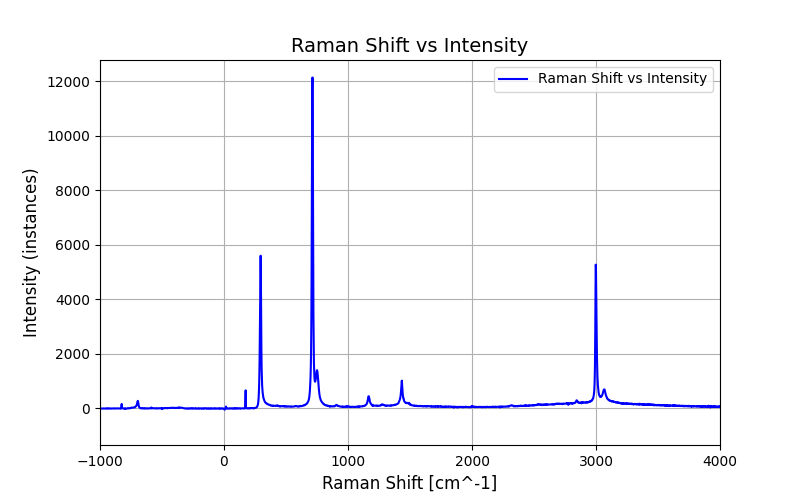
\includegraphics[width=\textwidth]{images/raman_spectra/raman_shift_DCM.png}
        \caption{Experimental Raman spectrum of dichloromethane}
        \label{fig:dcm_x}
    \end{figure}

    \begin{figure}[h]
        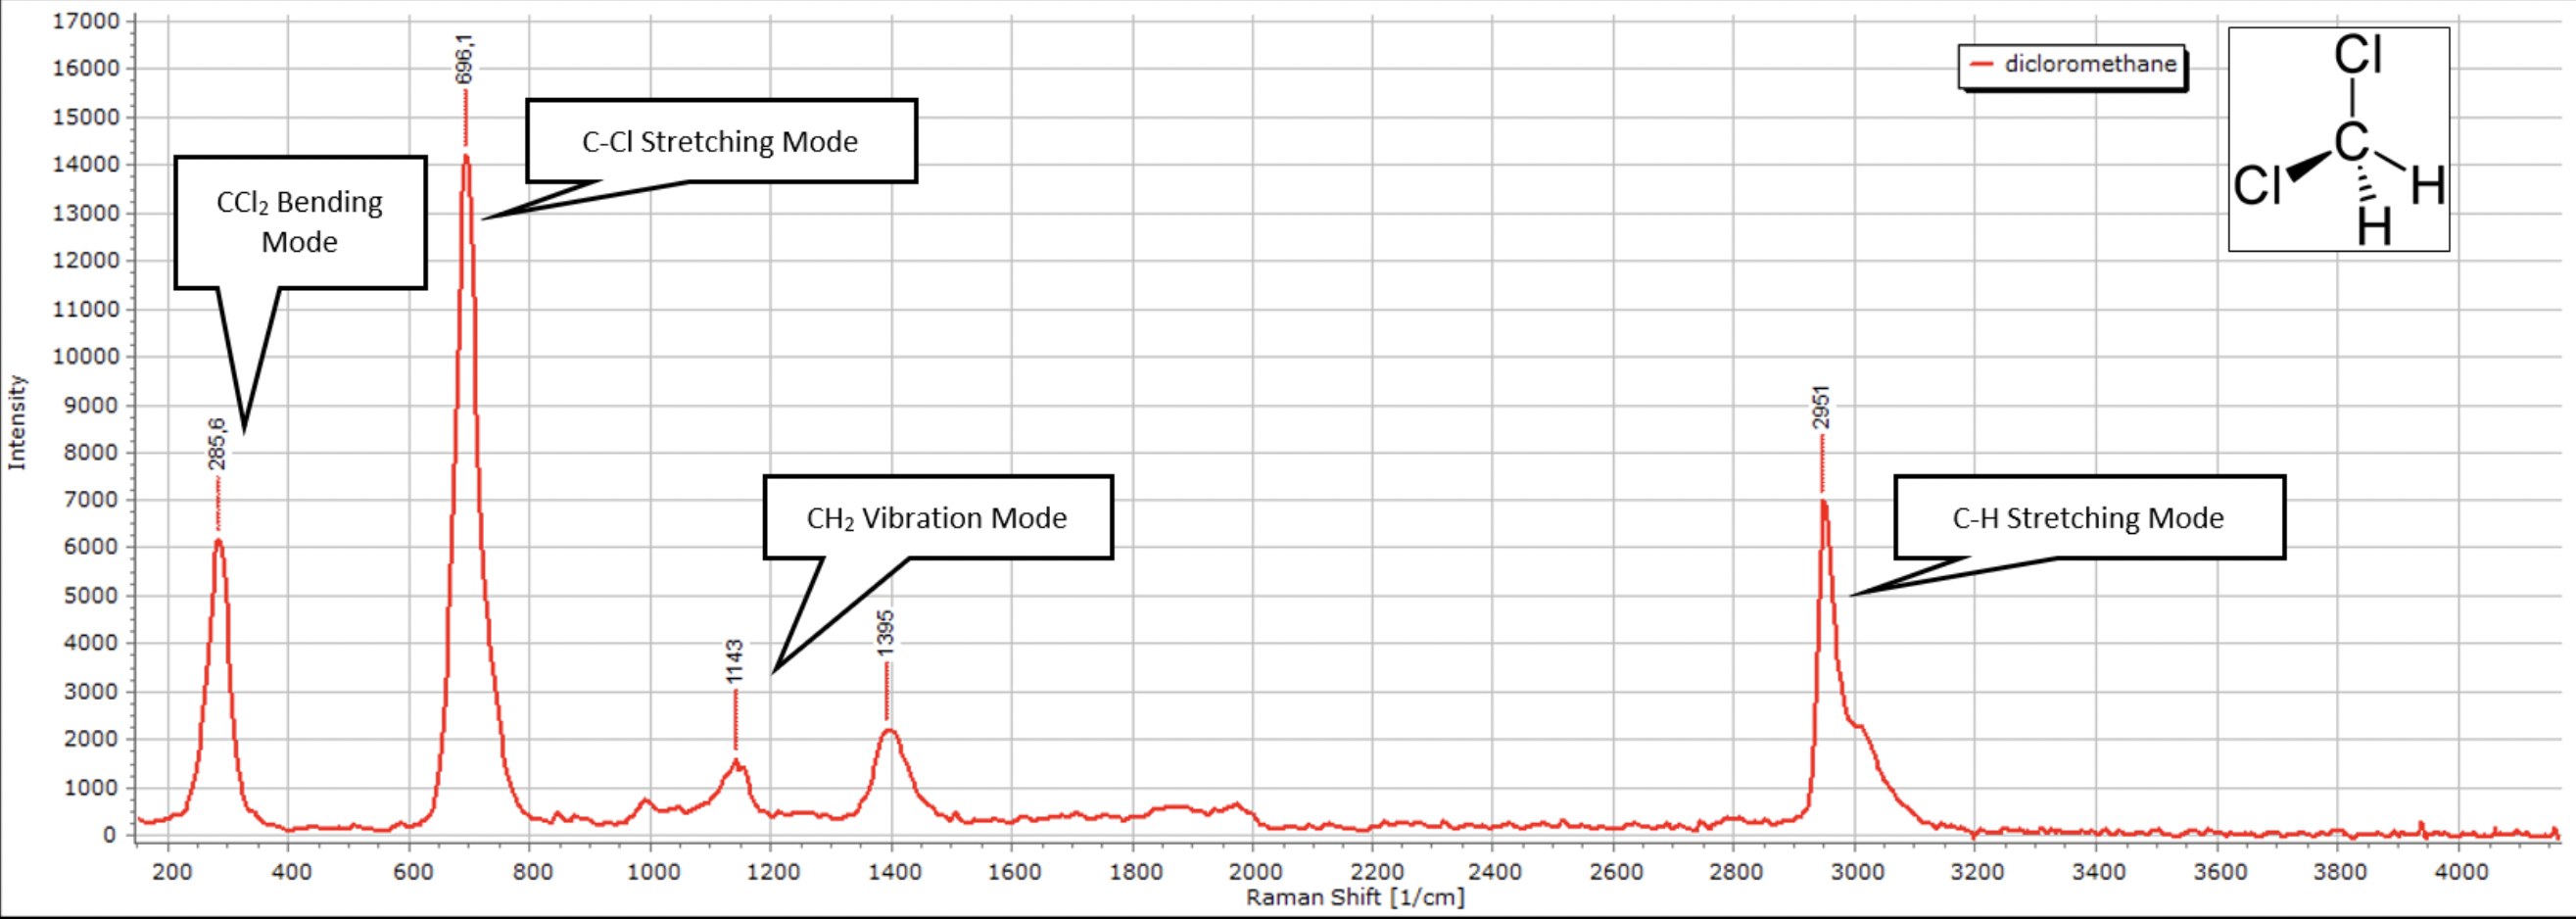
\includegraphics[width=\textwidth]{images/lit_raman/dichloromethane.png}
        \caption{Literature Raman spectrum of dichloromethane \cite{spectrumdcm}}
        \label{fig:dcm_l}
    \end{figure}

    \newpage

    Figure \ref{fig:eth_x} shows the experimentally aquired Raman spectrum of ethanol, with peaks at 442 nm, 894 nm, 1064 nm, 1107 nm, 1287 nm, 1465 nm, 2891 nm, 2942 nm and 2985 nm.

    \newpage

    \begin{figure}[h]
        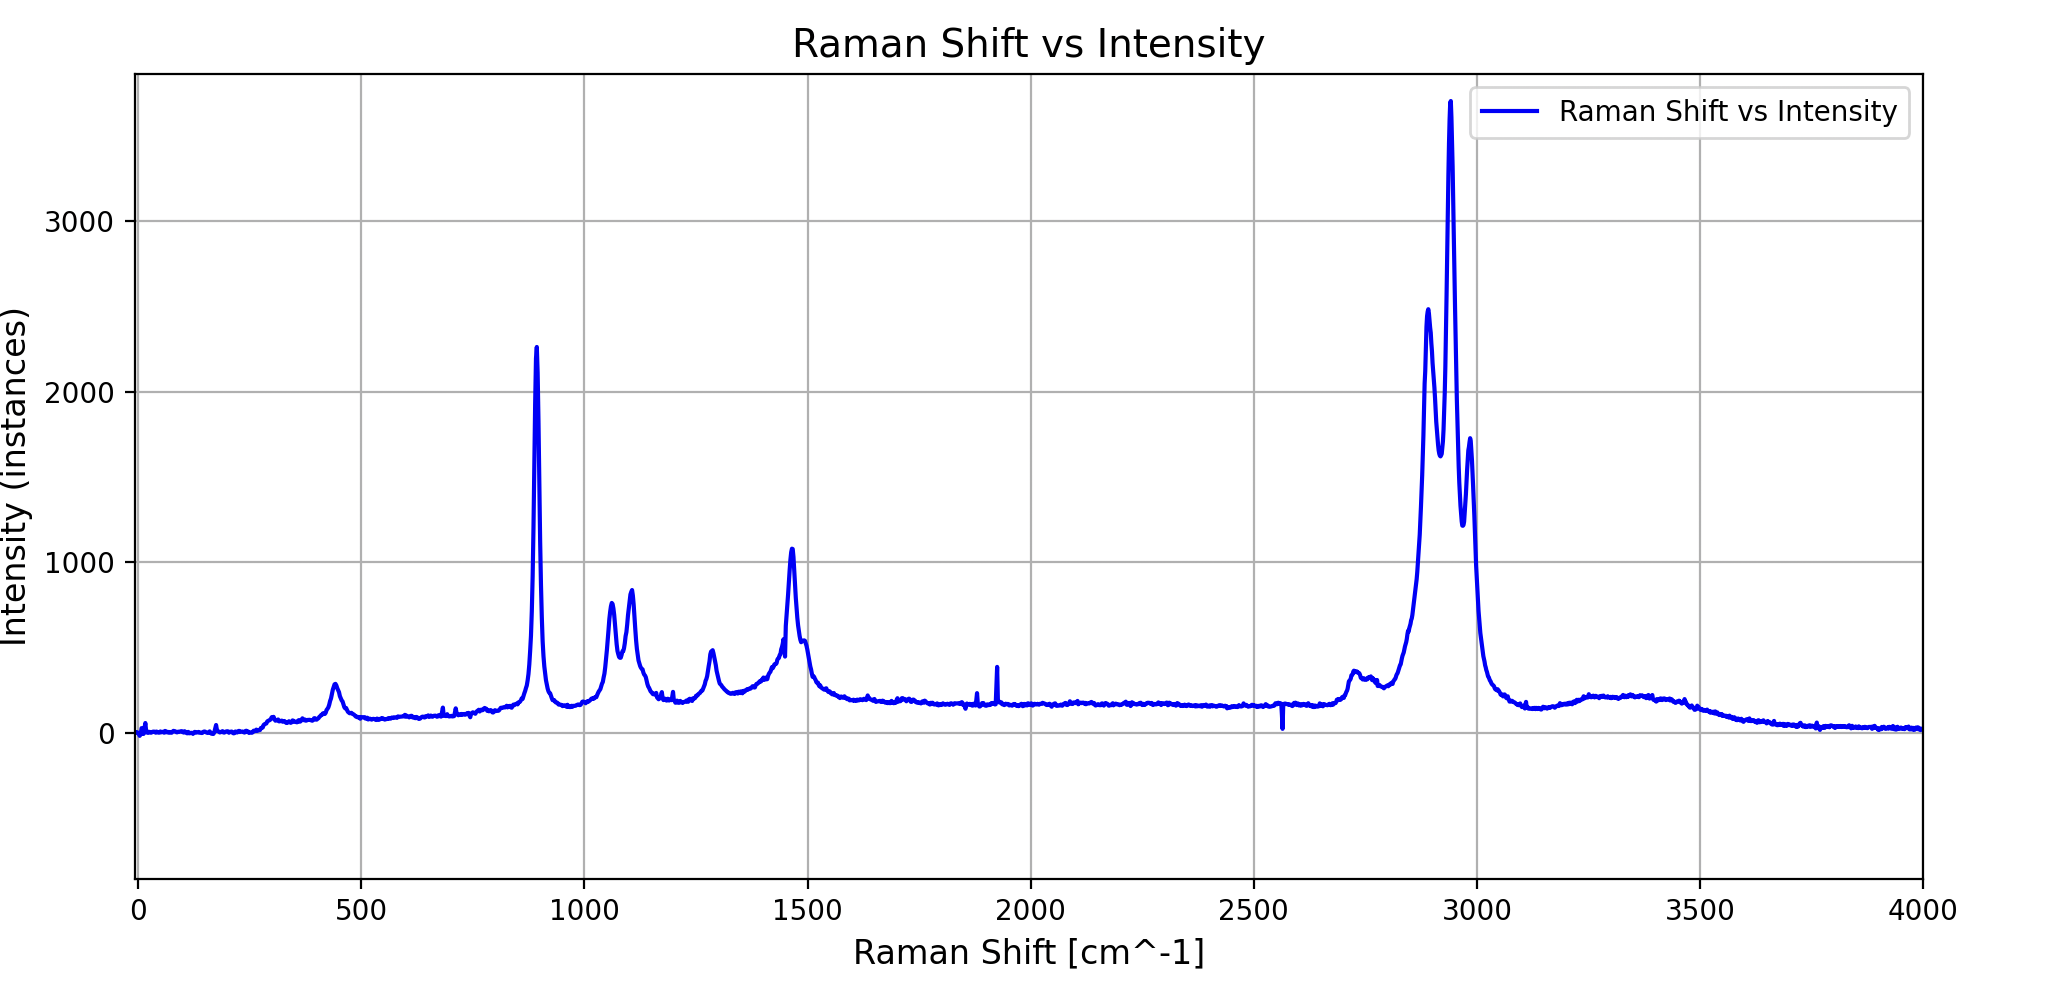
\includegraphics[width=\textwidth]{images/raman_spectra/raman_shift_ethanol.png}
        \caption{Experimental Raman spectrum of ethanol}
        \label{fig:eth_x}
    \end{figure}

    \begin{figure}[h]
        \centering
        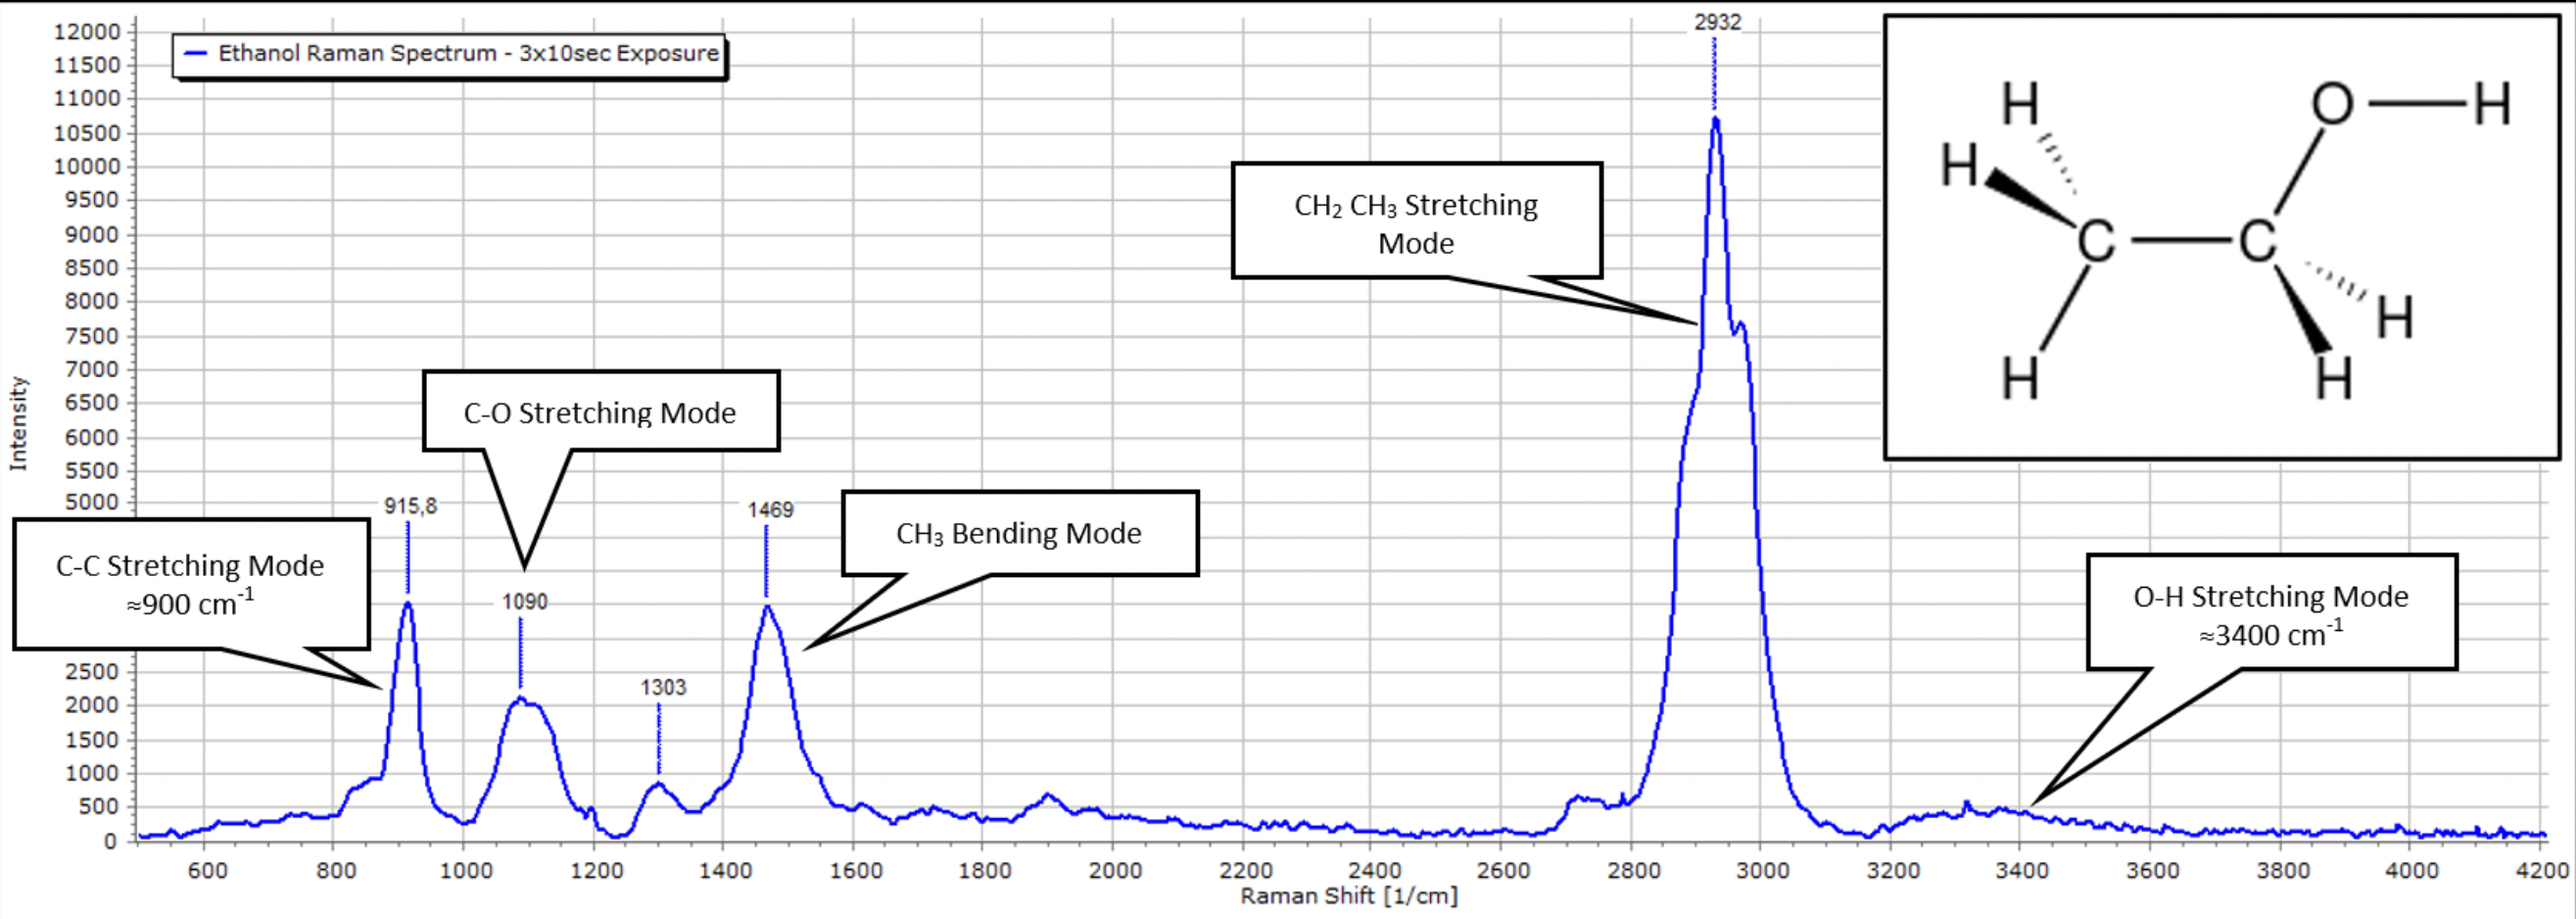
\includegraphics[width=\textwidth]{images/lit_raman/ethanol.png}
        \caption{Literature Raman spectrum of ethanol \cite{spectrumeth}}
        \label{fig:eth_l}
    \end{figure}

    \newpage

    Figure \ref{fig:pe_x} shows the experimentally aquired Raman spectrum of polyethylene, with peaks at 175 nm, 1073 nm, 1139 nm, 1305 nm, 1451 nm, 1860 nm and 2893 nm.

    \newpage

    \begin{figure}[h]
        \centering
        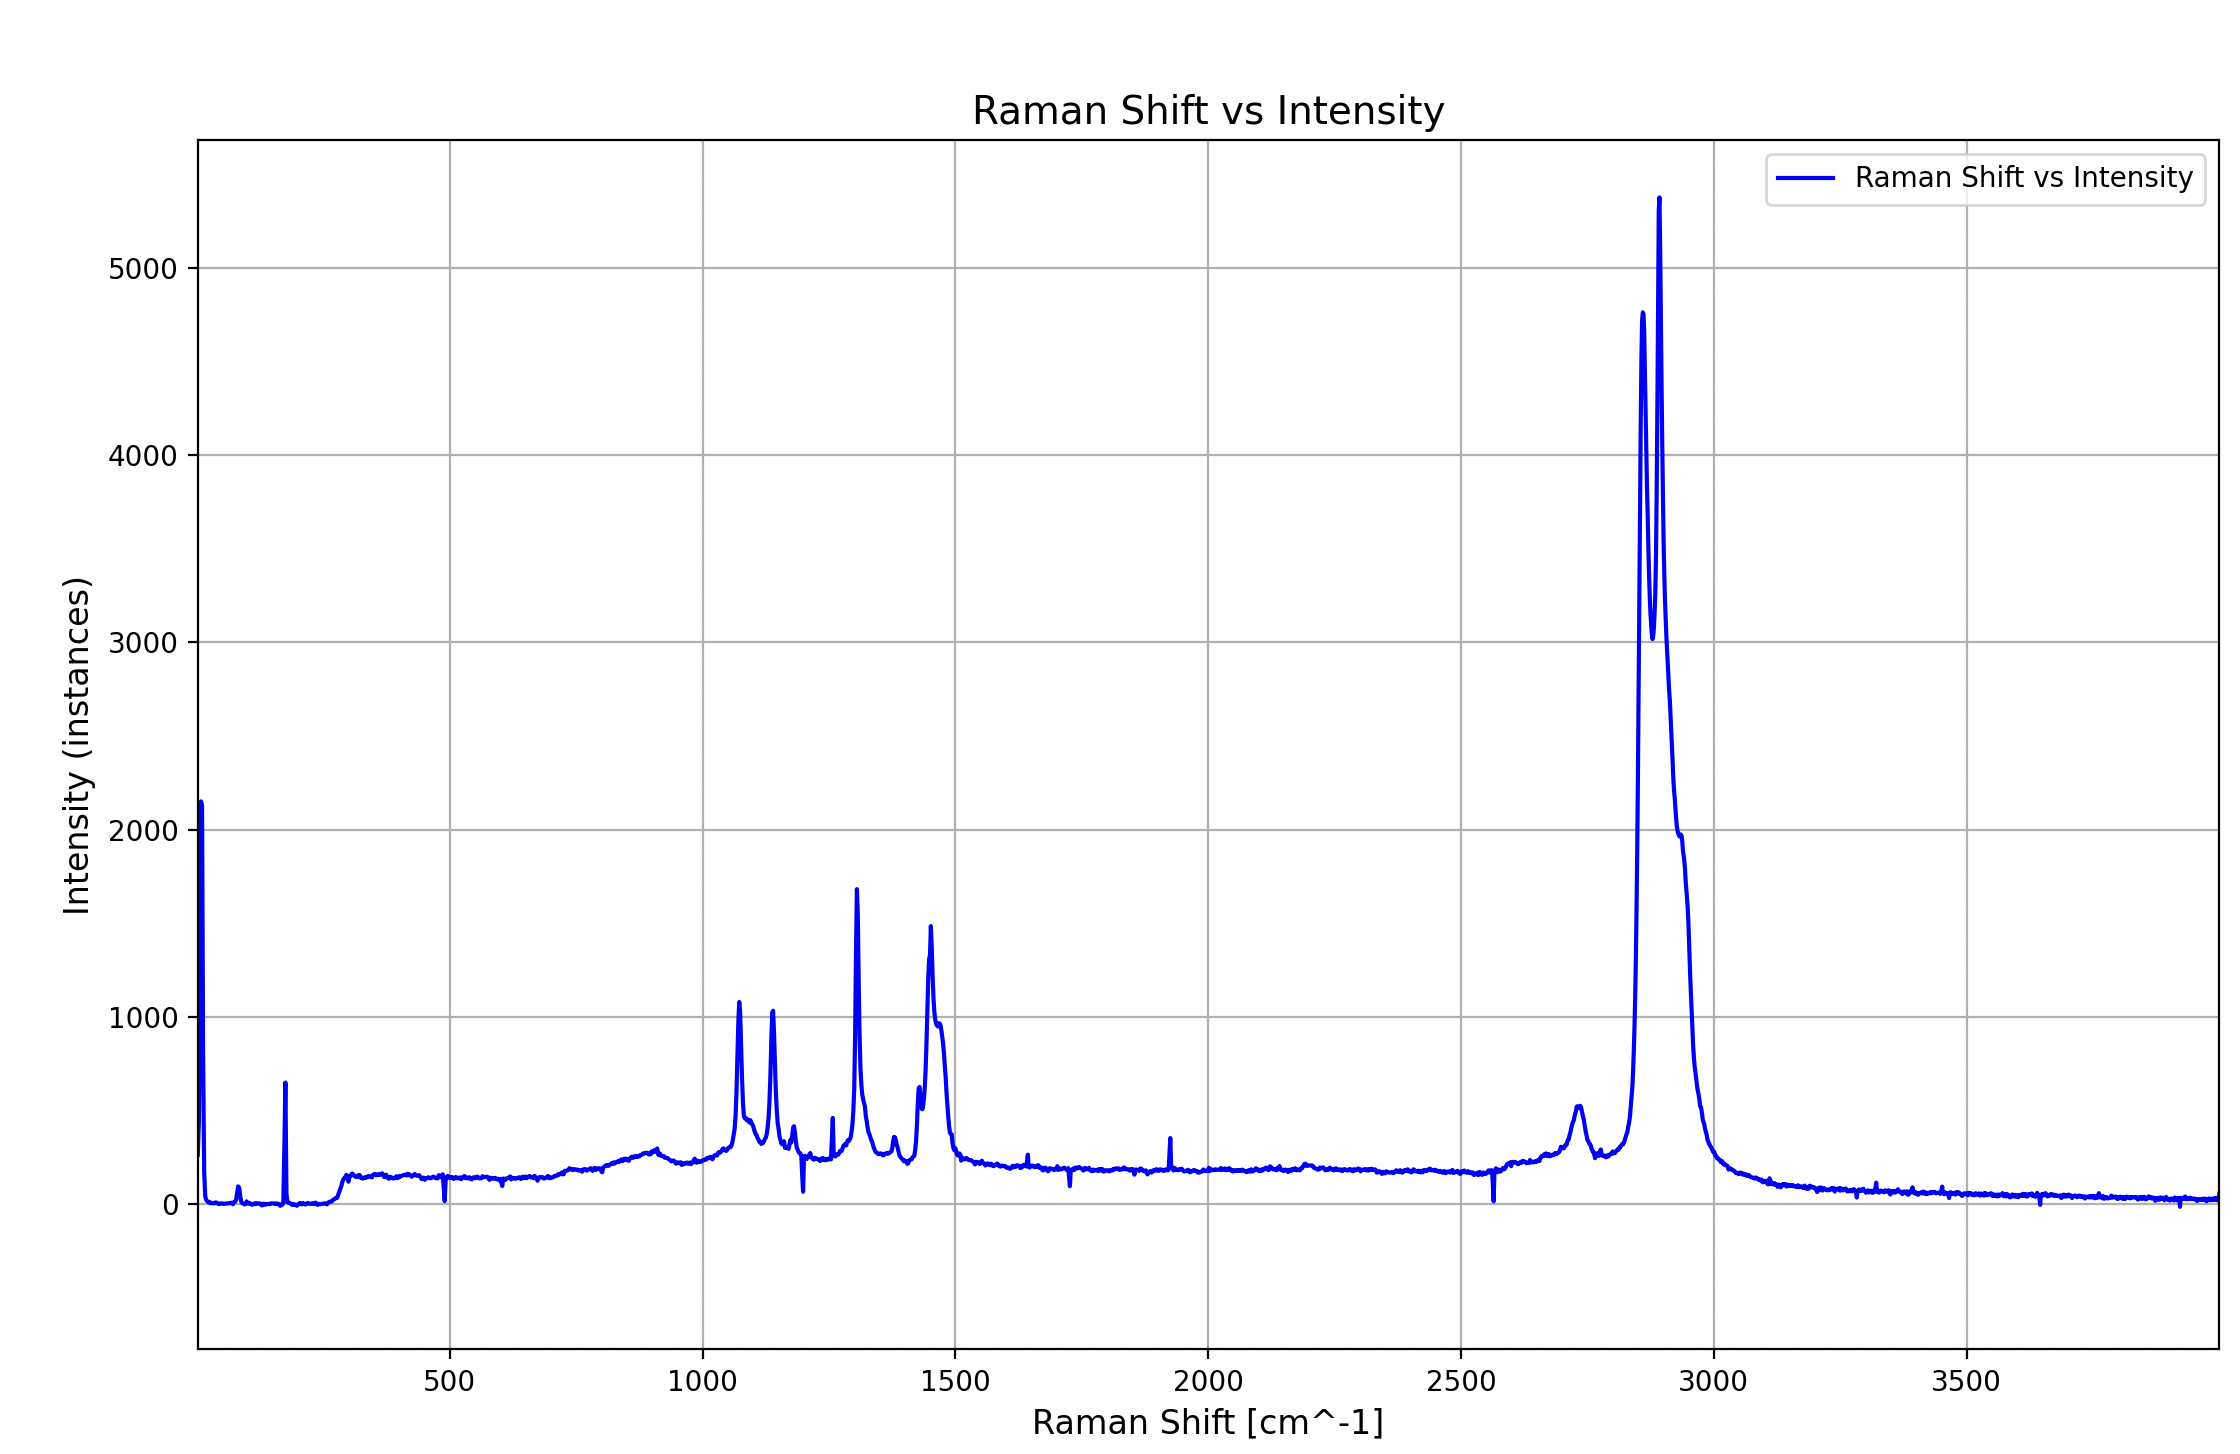
\includegraphics[width=\textwidth]{images/raman_spectra/raman_shift_polyethyleneh.png}
        \caption{Experimental Raman spectrum of polyethylene}
        \label{fig:pe_x}
    \end{figure}

    \begin{figure}[h]
        \centering
        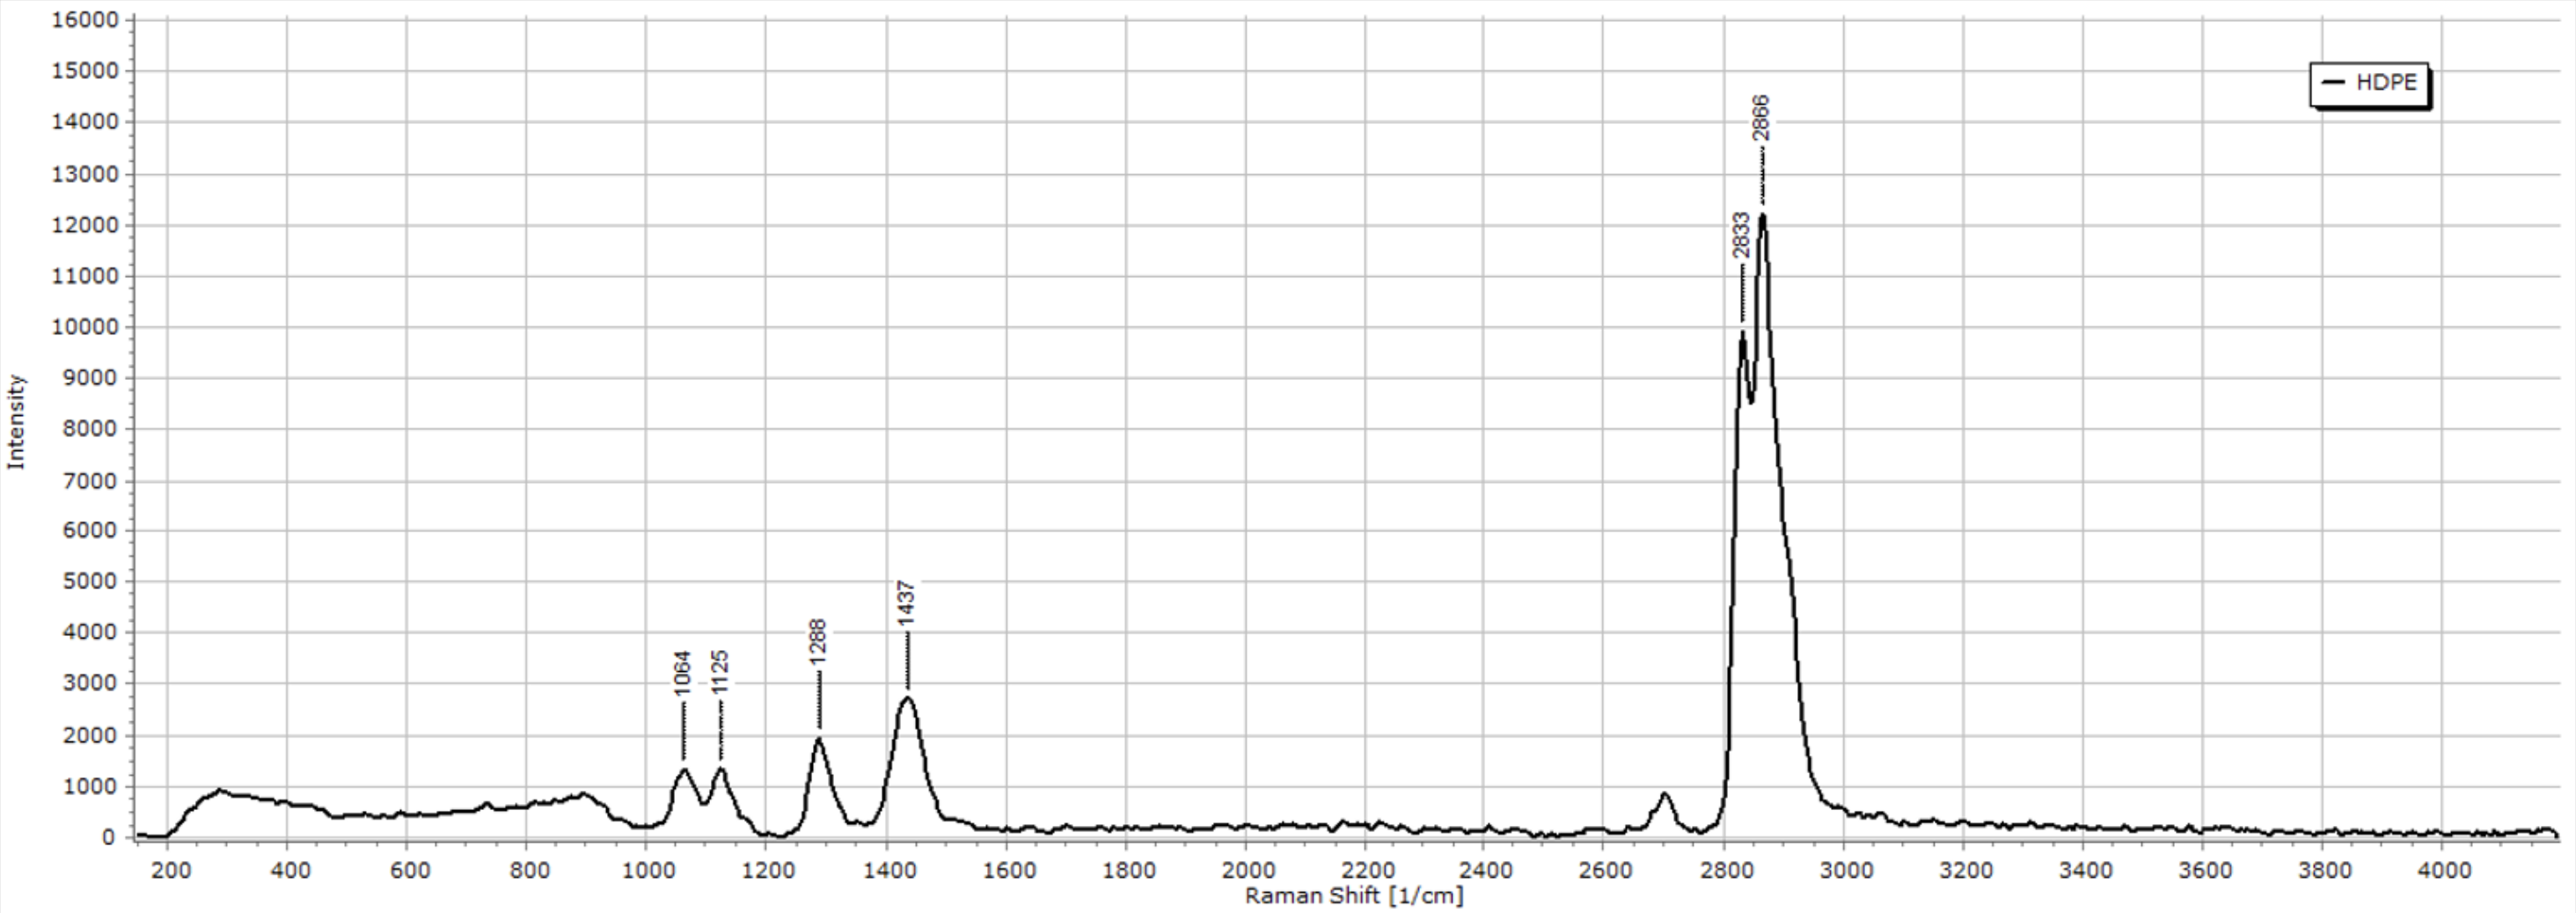
\includegraphics[width=\textwidth]{images/lit_raman/HDPE.png}
        \caption{Literature Raman spectrum of polyethylene \cite{spectrap}}
    \end{figure}

    \newpage

    Figure \ref{fig:ps_x} shows the experimentally aquired Raman spectrum of polystyrene, with peaks at 631 nm, 805 nm, 1012 nm, 1210 nm, 1337 nm, 1461 nm, 1613 nm, 2864 nm, 2917 nm and 3068 nm.

    \newpage

    \begin{figure}[h]
        \centering
        \makebox[\textwidth][c]{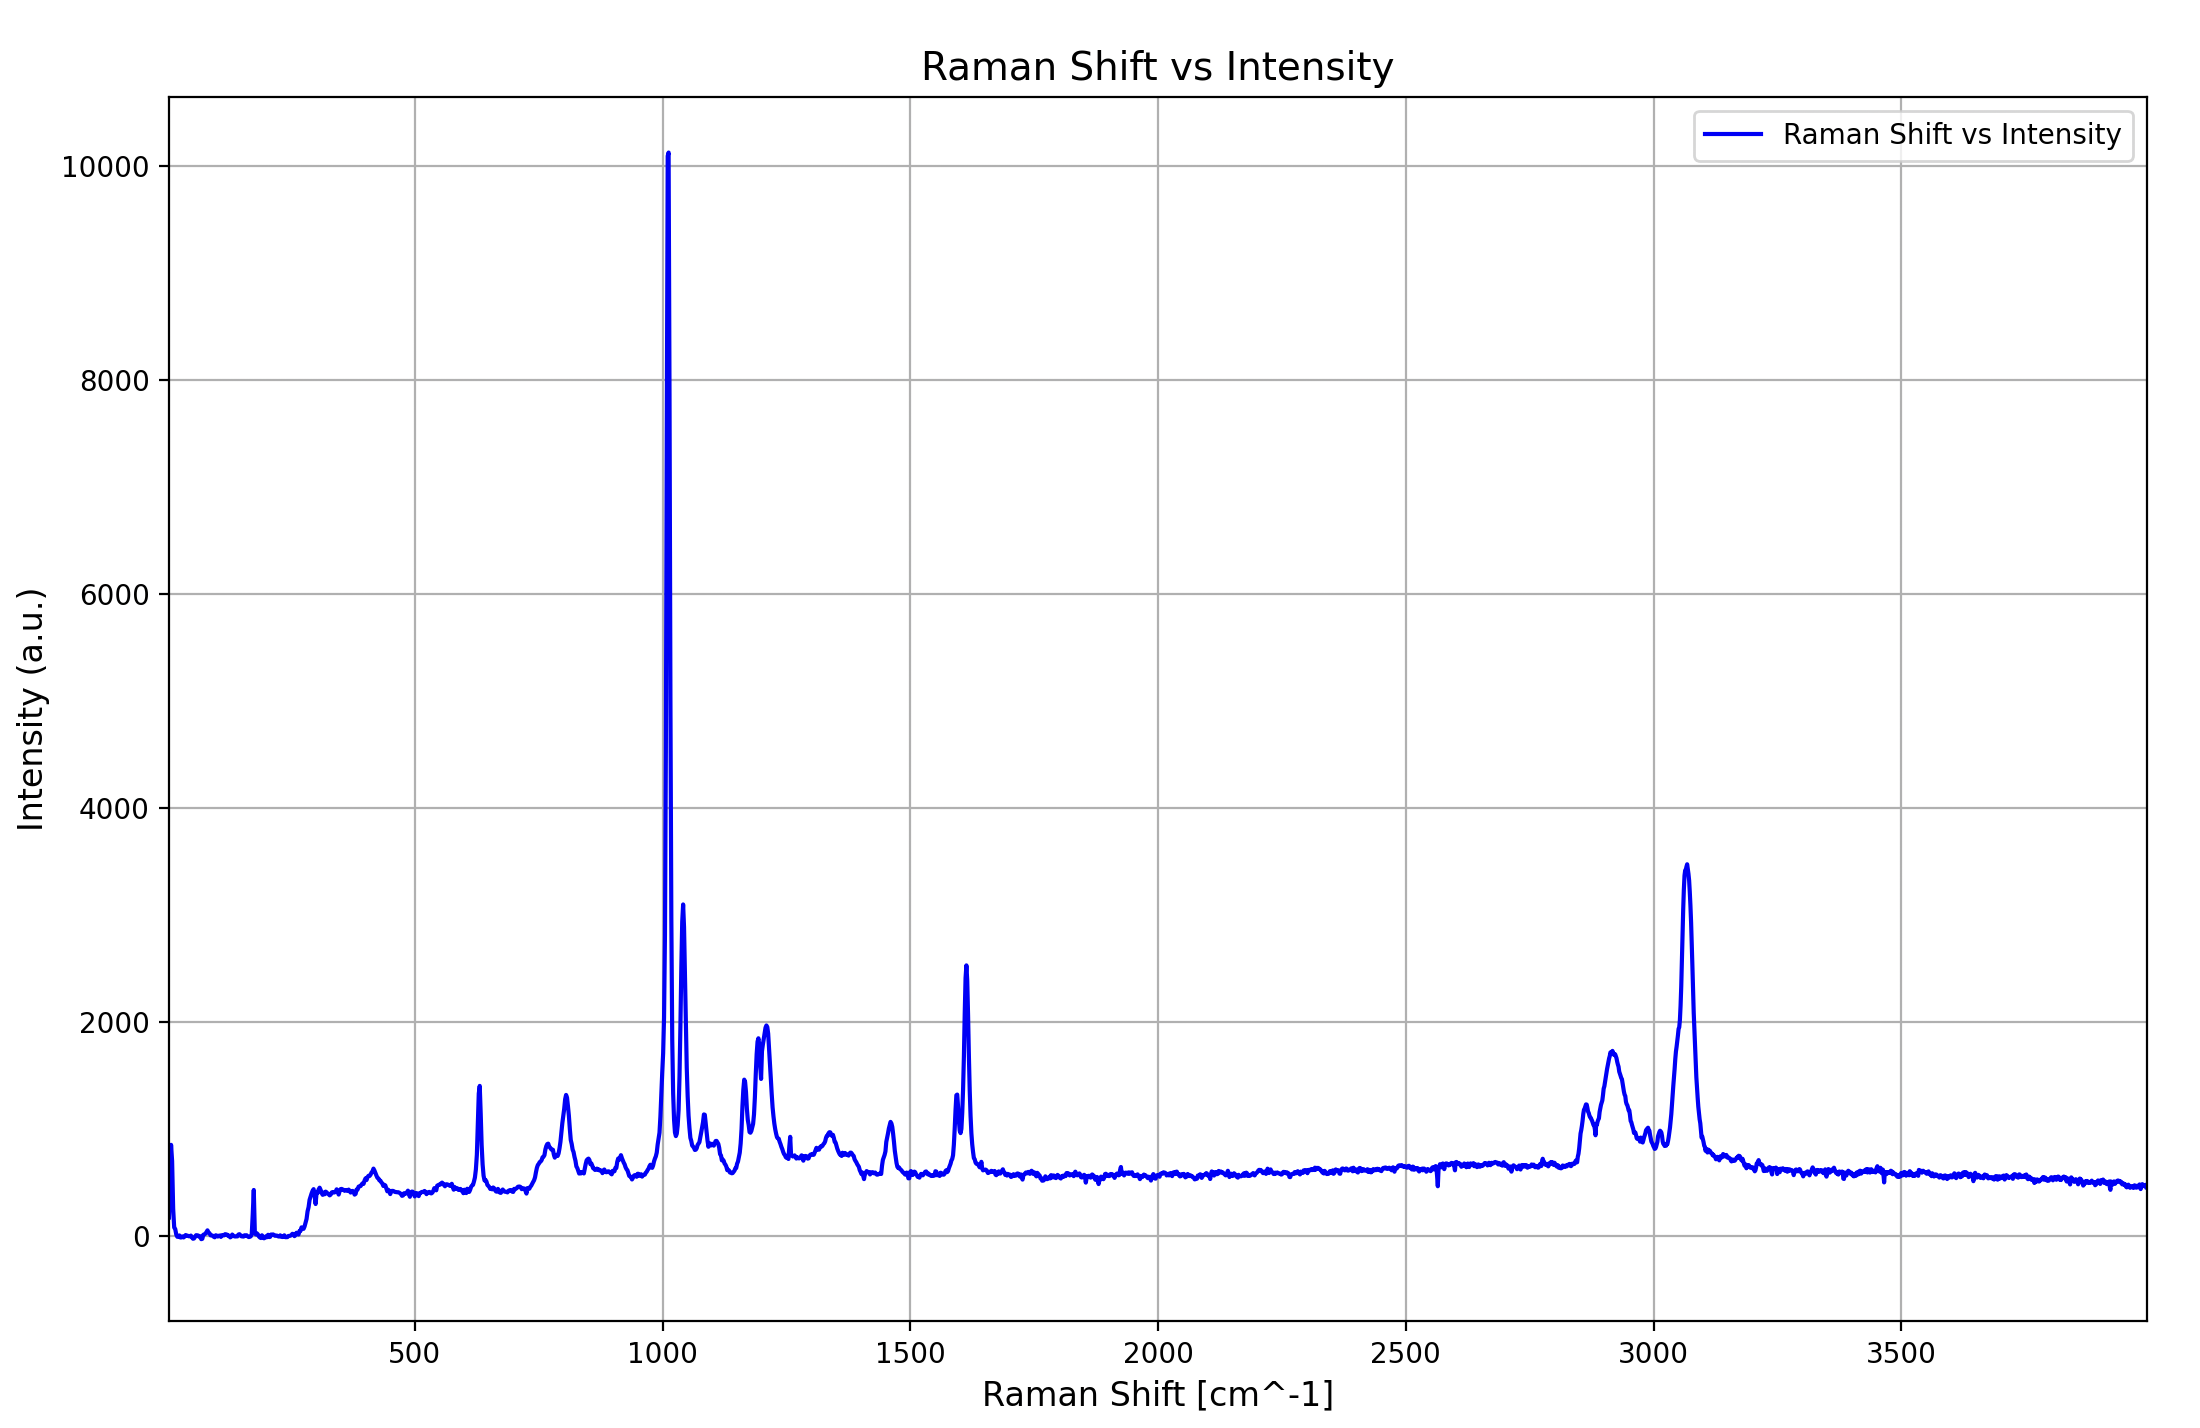
\includegraphics[width=1.2\textwidth]{images/raman_spectra/raman_shift_polystyreneh.png}}
        \caption{Experimental Raman spectrum of polystyrene}
        \label{fig:ps_x}
    \end{figure}

    \begin{figure}[h]
        \centering
        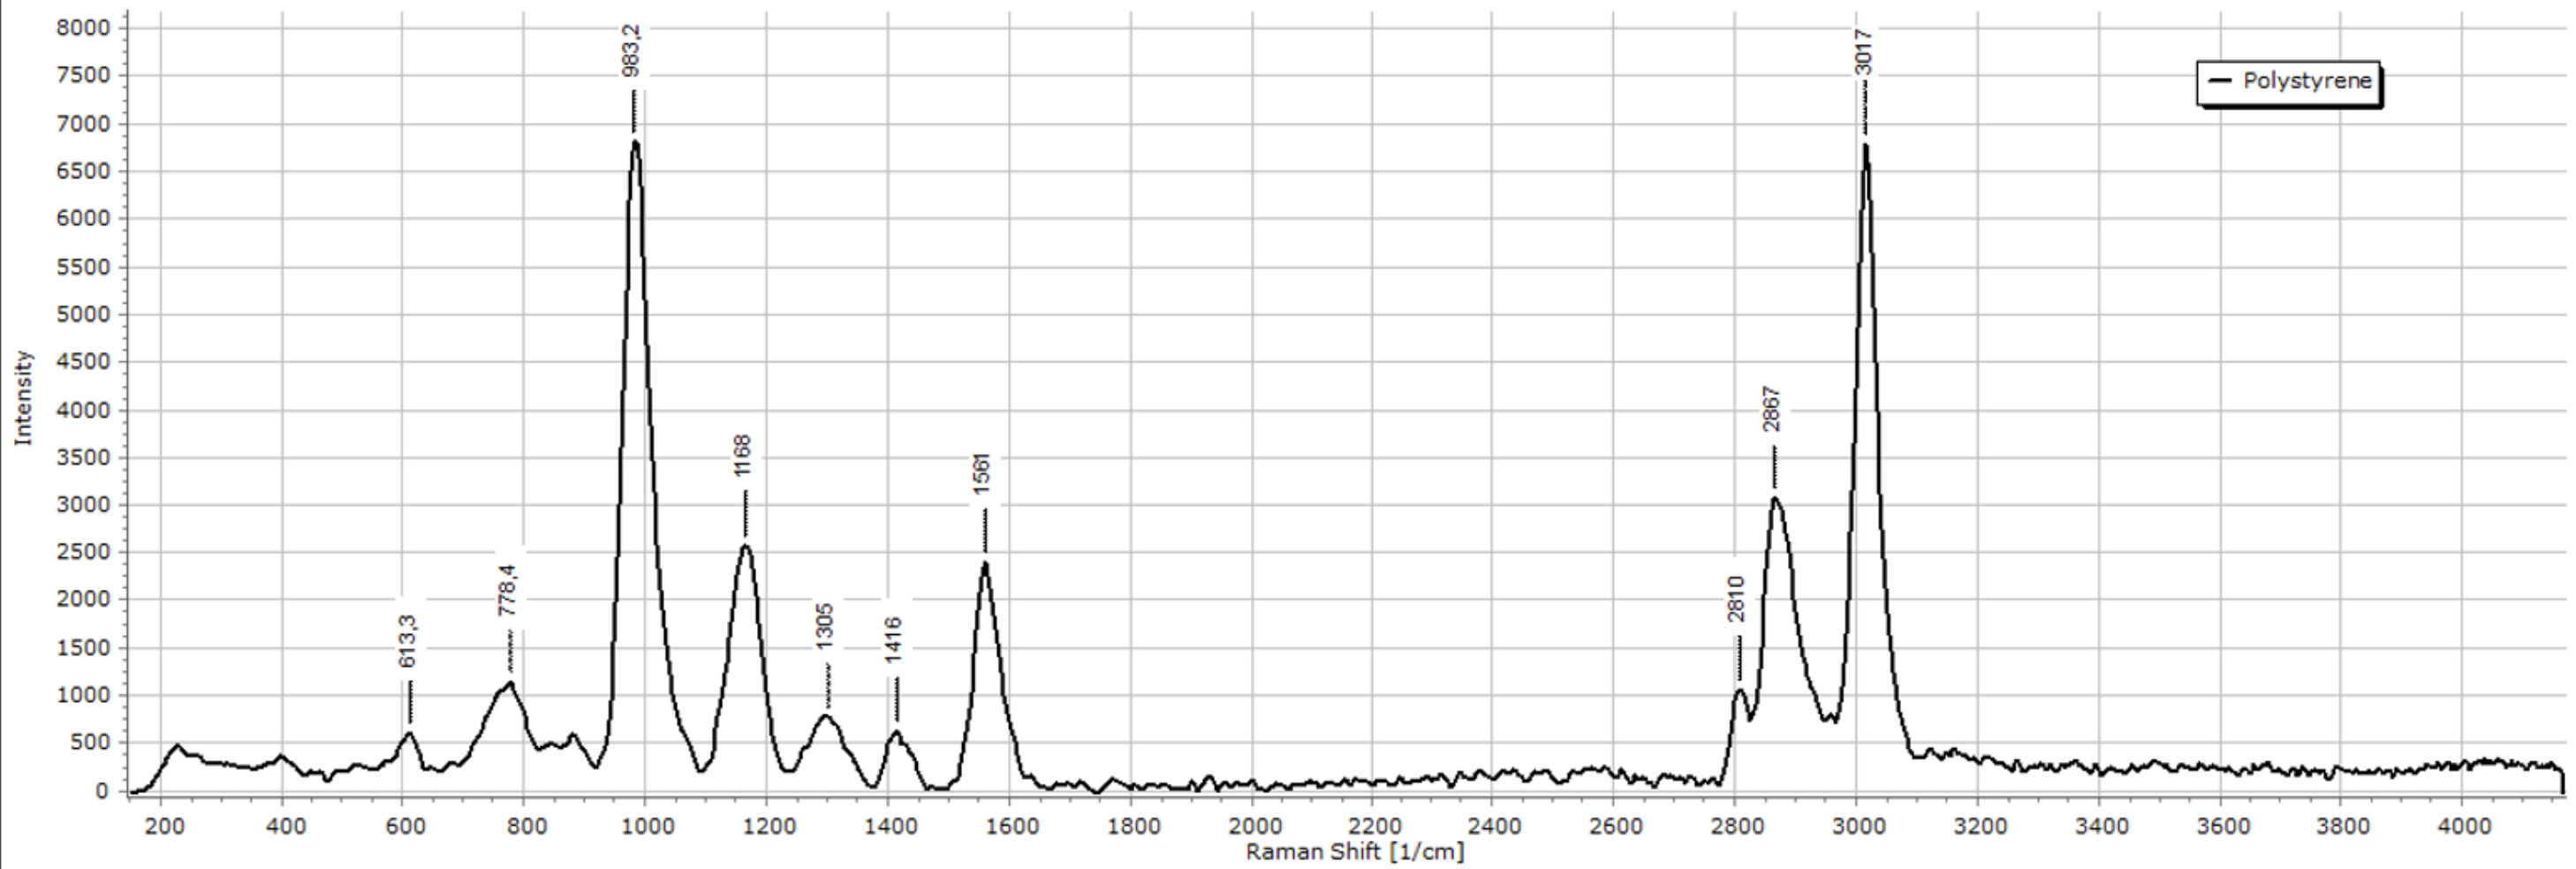
\includegraphics[width=\textwidth]{images/lit_raman/PS.png}
        \caption{Literature Raman spectrum of polystyrene \cite{spectrap}}
    \end{figure}
